

\StartOf{Lecture 1}

\Today{(1) Syllabus (2) Intro to Digital Communications}

\section{About My Notes}


I type my lecture notes.  My previous version of these lecture notes for my entire spring 2019 course is on Canvas.  I will be updating my notes each time I give a lecture, even up to the lecture time.   I will post my updated lecture notes online, which you can use after lecture to help you follow the lecture.  However, you must accept these conditions:
\begin{enumerate}
 \item \textbf{Taking notes is important}: I find most learning requires your active recording, not just watching.  Please take your own notes.  I have a big right margin on my notes, so you have room to copy your own notes next to mine.
 \item \textbf{My written notes do not and cannot reflect everything said during lecture}:  I answer questions and understand your perspective better after hearing your questions, and I try to tailor my approach during the lecture.  If I didn't, you could just watch a recording.
\end{enumerate}


\section{Introduction}

A digital communication system conveys discrete-time,
discrete-valued information across a physical channel.  Information
sources might include audio, video, text, or data.  They might be
continuous-time (analog) signals (audio, images) and even 1-D or
2-D.  Or, they may already be digital (discrete-time,
discrete-valued).  Our object is to convey the signals or data to
another place (or time) with as faithful representation as possible.

In this section we talk about what we'll cover in this class, and
more importantly, what we won't cover.

\subsection{``Executive Summary''}

Here is the one sentence version:  {\bf We will study how to efficiently encode digital data on a noisy analog medium, without interfering with other signals sent on the same medium, so that decoding the data (\ie, reception) at a receiver is simple, efficient, and high-fidelity.}

The keys points stuffed into that one sentence are:
\begin{enumerate}
 \item Digital information on an analog medium:  We can send analog signals, \ie, real-valued, continuous-time functions, on the medium.  The medium is, for example, EM waves on the air, EM waves in an optical fiber, magnetic field on a drive.  It is also called a ``channel''.  The signals sent on the medium are composed of waveforms.  In particular, we will send {\bf linear combinations of orthogonal waveforms}.  In digital communications systems, there are a discrete list of possible linear combinations we might send, one for each possible symbol.  We will discuss why and what linear combinations, and what orthogonal waveforms are and why they are useful.
 %
 \item Decoding the data:  When receiving a signal (a function) in noise, it will not match exactly what was sent.  How should a receiver make a decision about which signal was sent?
 %
 \item What makes a receiver difficult to realize?  What choices of waveforms make a receiver simpler to implement?  What techniques are used in a receiver to compensate?
 %
 \item Efficiency, Bandwidth, and Fidelity:  Fidelity is the correctness of the received data (\ie, the opposite of error rate).  What is the tradeoff between energy, bandwidth, and bit error rate?  We want all three to be low (low consumption, low bandwidth usage, and low bit error rate).  Energy and bandwidth are the costs of our communication system, and fidelity is how well it performs.
\end{enumerate}
You can look at this like an impedance matching problem from circuits.  You want, for power efficiency, to have the source impedance match the destination impedance.  In digital comm, this means that we want our waveform choices to match the channel and receiver to maximize the efficiency of the communication system.



\subsection{Why not Analog?}

Analog systems still exist and will continue to exist; however, new systems you will design during your career will almost always be digital communication systems. Why?
\begin{itemize}
  \item Fidelity: Analog systems will always have noise in the received signal.  Digital communications systems can be designed to achieve an arbitrarily low error rate.
  \item Energy: transmit power, and device power consumption
  \item Bandwidth efficiency: digital communications systems can be significantly more efficient in use of the spectrum than older analog systems.
  \item Moore's Law decreases device costs for digital hardware
  \item Increasingly the information needed to be transferred is fundamentally digital
  \item More powerful information security is possible
\end{itemize}

\subsection{Networking Stack}

In this course, we study digital communications from bits to bits.  That is, we study how to take ones and zeros from a transmitter (TX), send them through a medium, and then (hopefully) correctly identify the same ones and zeros at the receiver (RX).  There's a lot more than this to the digital communication systems which you use on a daily basis (\eg, cellular phone, Wi-Fi, Bluetooth, wireless keyboard, wireless car key).

To manage complexity, we (engineers) don't try to build a system to do everything all at once.  We typically start with an application, and we build a layered network to handle the application.  Each layer has particular inputs and outputs that are standardized so that we can change the operation of one layer (ideally) without change to the other layers.  The 7-layer OSI stack, which you would study in a CS computer networking class, is as follows:
\begin{itemize}
  \item Application
  \item Presentation $\star$
  \item Session $\star$
  \item Transport
  \item Network
  \item Link Layer
  \item Physical (PHY) Layer
\end{itemize}
(Note that there is also a 5-layer model in which $\star$ layers are
considered as part of the application layer.)  ESE 471 is part of
the bottom layer, the physical layer. In fact, the physical layer
has much more detail. It is primarily divided into:
\begin{itemize}
  \item Multiple Access Control (MAC)
  \item Encoding
  \item Channel / Medium
\end{itemize}
We can control the MAC and the encoding chosen for a digital
communication.

\subsection{Channels and Media}

We can chose from a few media, but we largely can't change the
properties of the medium (although there are exceptions). Here are
some media:
\begin{itemize}
  \item Wireless EM Media: (anything above 0 Hz) Radio, Microwave, mm-wave
  bands, light
  \item Acoustic:  ultrasound
  \item Wired EM Media: Transmission lines, waveguides, optical fiber, coaxial
  cable, wire pairs, ...
  \item Disk (data storage applications)
\end{itemize}

\subsection{Encoding / Decoding Block Diagram}

\begin{figure}[htbp]
  \includegraphics[width=\textwidth]{../images/Tx-Channel-Rx-Block-Diagram.eps}
  \caption{Block diagram of a single-user digital communication system, including (top) transmitter (TX), (middle) channel, and (bottom) receiver (RX).}
  \label{F:Tx-Rx-Blocks}
\end{figure}

Notes:
\begin{itemize}
  \item Information source comes from higher networking layers.  It
  may be continuous or packetized.
  %
  \item Source Encoding:  Finding a compact digital representation for
  the data source.  Includes sampling of continuous-time signals,
  and quantization of continuous-valued signals.  Also includes
  compression of those sources (lossy, or lossless).  What are some
  compression methods that you're familiar with? 
  %
  \item Channel encoding refers to redundancy added to the signal
  such that some bit errors can be later be corrected by the channel decoder.  
  %
  \item Modulation refers to the digital-to-analog conversion which
  produces a continuous-time signal that can be sent on the physical
  channel.  It is analogous to impedance matching - proper matching of a
  modulation to a channel allows optimal information transfer, like impedance
  matching ensured optimal power transfer.    Modulation and demodulation
  will be the main focus of this course.
  %
  \item Channels: See above for examples.  Typical models are
  additive noise, or linear filtering channel.
\end{itemize}

Why do we do both source encoding (which compresses the signal as
much as possible) and also channel encoding (which adds redundancy
to the signal)?  Shannon's source-channel coding
separation theorem says that (given enough time) we can do both and yet
consider them separately, without any loss.  And separation,
like layering, reduces complexity to the designer.  We will introduce source and channel encoding and decoding towards the end of this semester.  Each could be (and is) a semester course in itself.


\subsection{Channels}

A channel can often be modeled as a linear filter with the
addition of noise.  The noise comes from a variety of sources, but
predominantly:
\begin{enumerate}
  \item Thermal background noise:  Due to the physics of living
  above 0 Kelvin.  Well modeled as Gaussian, and constant across frequency.  It is
  commonly referred to as additive white Gaussian noise (AWGN).  The ``white'' color moniker comes from being constant across frequency, however, note that white, gray, and black are all colors
  that are constant across frequency.  I will typically refer to the noise as ``additive uncorrelated Gaussian'' which I feel is more precise.
  \item Interference from other transmitted signals.  These other
  transmitters whose signals we cannot completely cancel, we lump
  into the `interference' category.  These may result in non-Gaussian
  noise distribution, and  noise spectral density that varies with frequency.
\end{enumerate}
The linear filtering of the channel results from the physics and EM
of the medium.  For example, attenuation in telephone wires varies
by frequency.  Narrowband wireless channels experience fading that
varies as a function of frequency.  Wideband wireless
channels display multipath, due to multiple time-delayed
reflections, diffractions, and scattering of the signal off of the
objects in the environment.  All of these can be modeled as linear
filters.  

The filter may be constant, or time-invariant, if the medium, the TX
and RX do not move or change.  There may be slow movement of the TX or RX which causes the
channel may change slowly over time.  Even for a stationary TX
and RX, in real wireless channels, movement of cars, people, trees,
etc. in the environment may change the channel slowly over time.  For rapidly movement in a wireless channel, we will experience Doppler spreading, which is a non-linear effect, in which case our channel is neither linear nor time-invariant.

\begin{figure}[htbp]
  \centerline{\includegraphics[width=\textwidth]{../images/Channel-Detail-Diagram.eps}}
  \caption{Linear filter and additive noise channel model.}
  \label{F:Channel-Blocks}
\end{figure}

In this course, we will focus primarily on the additive noise channel, but we
will mention what variations exist for particular channels, and how
they are addressed.

\subsection{Topic:  Random Processes}

What are things that can be considered random in a communication system?

\Solution{
Random things in a communication system:
\begin{itemize}
  \item Noise in the channel
  \item Signal (bits)
  \item Channel filtering, attenuation, and fading
  \item Device frequency, phase, and timing offsets
\end{itemize}
These random signals often pass through LTI filters, and are
sampled.  
}

We want to build the best receiver possible despite the random impediments.  Optimal
receiver design is something that we study using probability theory.

We have to tolerate errors.  Noise and attenuation of the channel
will cause bit errors to be made by the demodulator and even the
channel decoder.  This may be tolerated, or a higher layer
networking protocol (\eg, TCP) can determine that an error
occurred and then re-request the data.

\subsection{Topic:  Frequency Domain Representations}

To fit as many signals as possible onto a channel, we often split
the signals by frequency.  The concept of sharing a channel is
called \emph{multiple access} (MA).  Separating signals by frequency
band is called frequency-division multiplexing (FDM) or frequency domain multiple access (FDMA).  For the
wireless channel, this is controlled by the FCC (in the US) and
called spectrum allocation. There is a tradeoff between frequency
requirements and time requirements, which will be a major part of
this course.  The Fourier transform of our modulated, transmitted
signal is used to show that it meets the spectrum allocation limits
of the FCC.

\subsection{Topic:  Orthogonality and Signal Space}

To show that signals sharing the same channel don't interfere with
each other, we need to show that they are \emph{orthogonal}.  This
means, in short, that a receiver can uniquely separate them. Signals
in different frequency bands are orthogonal.

We can also employ multiple orthogonal signals in a single
transmitter and receiver, in order to provide multiple independent
means (dimensions) on which to modulate information.  We'll send signals that are orthogonal to the signals we send at a later time, so that we can convey different information over time and not have our own information signal interfere with itself.

We'll use signal spaces to show graphically the
results, as the example in Figure \ref{F:MPSK-signalSpaceDiagram}.  In general, we will evaluate the performance of systems which \emph{send and receive linear combinations of orthogonal signals} in order to convey digital information.

\begin{figure}[htbp]
  \centerline{
  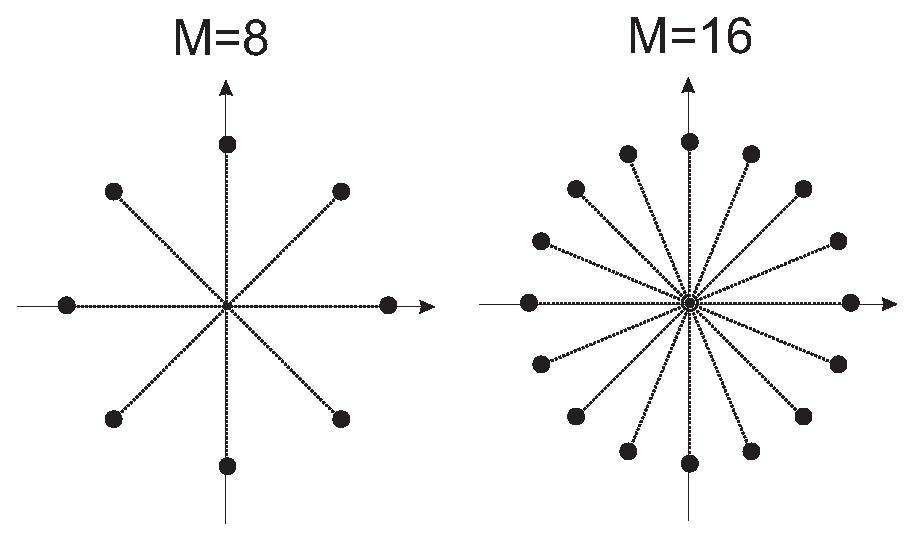
\includegraphics[width=0.8\textwidth]
  {../images/MPSK-signalSpaceDiagram.eps}
  }
  \caption{Example signal space diagram for $M$-ary Phase Shift Keying, for (a) $M=8$ and (b) $M=16$.
           Each point is a vector which can be used to send a 3 or 4 bit sequence.}
  \label{F:MPSK-signalSpaceDiagram}
\end{figure}

\subsection{Is there a need for Communications Engineers?}

Cisco's forecast (VNI Complete Forecast Highlights, \url{https://www.cisco.com/c/m/en_us/solutions/service-provider/vni-forecast-highlights.html}) says that we'll be sending 400 GB of data per capita in the US by next year, and IP traffic will triple every 5 years.  Mobile (wireless) traffic will increase twice as fast as wired.  We will not achieve these data rates using the same protocols that we have today.  Further the spectrum is well utilized; there is little additional bandwidth available to handle this rate of increase, so engineers will have to make communication systems more spectrum efficient, or make use of spectrum that is currently available at higher frequencies (20 GHz and above) where there is more spectrum available.  

Further the number of wireless devices we use are increasing rapidly.  These devices may have lower data rates (e.g., wireless thermostats) and should be able to operate with low energy consumption.  However today's  standard protocols (e.g., WiFi) do not allow them to operate in an energy efficient manner, and the protocols themselves operate inefficiently when serving large numbers of devices.  There will be multiple new generations of wireless protocols to handle our Internet-of-Things devices and allow them to be as efficient as they need to be.

Finally, the main objective of digital communications is to build systems in which we can reliably \emph{classify} information at a receiver.  A receiver must take in high-dimensional noisy measurements and make a decision about what is true about the information that was encoded.  Thus I argue that ESE 471 is the original course in ``big data''.  Information theory is still a fundamental tool in statistical machine learning, and digital communications is the background material for information theory.

%\subsection{Related classes}
%
%\begin{enumerate}
%\item Pre-requisites: Random Processes; Signals and Systems.
%\item Signal Processing:  Digital Signal Processing
%\item Electromagnetics:  EM Waves, Microwave Engineering, Antenna Theory, 
%\item Breadth: Wireless Communications Systems
%\item Devices and Circuits:  Fundamentals of Digital System Design, Analog IC Design \item Networking:  Embedded System Design,  Computer Networks
%\item Advanced Classes:  Software Radio, Information Theory,  Error Control Coding, Estimation Theory
%\end{enumerate}
